\chapter{晕 厥}

晕厥(syncope)是由于一过性全脑供血不足,导致急性发生的、短暂性的、自限性的意识丧失。患者因肌张力消失而倒地或不能维持正常姿势,可于短时间内恢复。意识丧失时间若超过10~20秒,有些患者可发生抽搐。

正常全脑血流量为800~1200ml/min,脑血流量受到下列因素影响:平均动脉压、平均静脉压、颅内压、脑血流阻力(主要是脑血管阻力和血液黏稠度)。也可用下列公式示之:


\includegraphics[width=2.57292in,height=1.11458in]{./images/Image00302.jpg}

此外,脑血流量的调节还受外周血管阻力、心率、血压以及压力感受器、化学感受器有关的神经体液影响。据估计维持意识所需的脑血流量的临界水平为30ml/(100g·min),当脑的灌注压降低50\%~55\%,即降至45~60mmHg时可发生晕厥;或者是当每100g脑组织的氧供应从114ml降到35ml时,持续8秒就会发生晕厥,如超过10~20秒可发生抽搐。

导致脑血流量骤减的原因是:①血压急剧下降;②心排出量突然减少;③供应脑部血流的动脉发生急性较广泛的缺血。引起这三种情况的可有:心律失常、心泵衰竭、静脉回流不全、微动脉张力缺失、血容量不足、神经-体液调节障碍。这些因素相互联系、相互作用。另外,引起③的因素还可有:动脉本身病变导致管腔狭窄或闭塞、颈部疾病或人为地压迫颈部血管、交感神经受累引起反射性椎动脉痉挛等。

\section{【晕厥疾病的分类】}

临床上可将晕厥分为三大类,即神经介导性晕厥(反射性晕厥)、直立性低血压性晕厥、心脏性晕厥(表\ref{tab48-1})。

\begin{longtable}{c}
 \caption{晕厥疾病的分类}
 \label{tab48-1}
 \endfirsthead
 \caption[]{晕厥疾病的分类}
 \endhead
 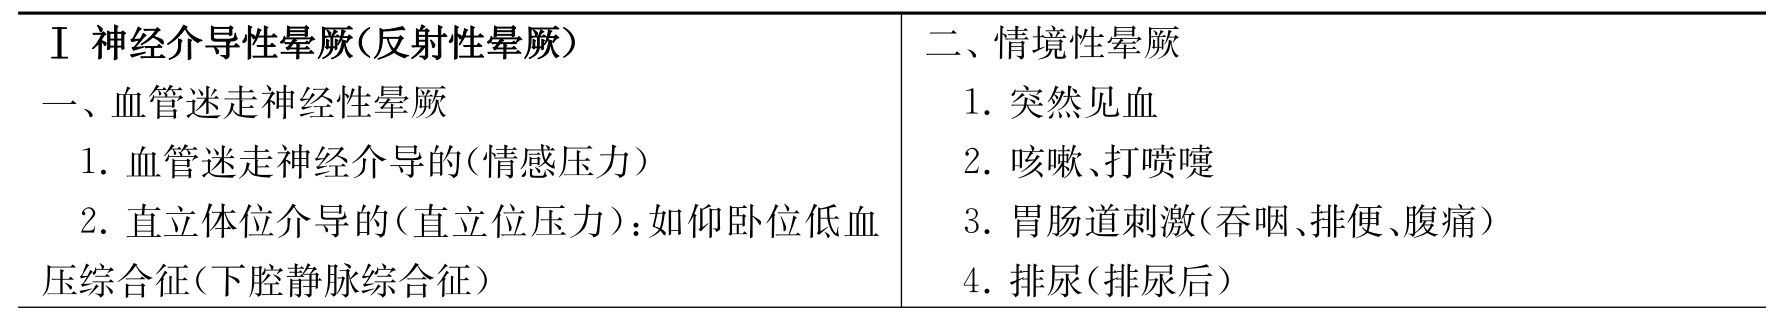
\includegraphics[width=\textwidth,height=\textheight,keepaspectratio]{./images/Image00303.jpg}\\
 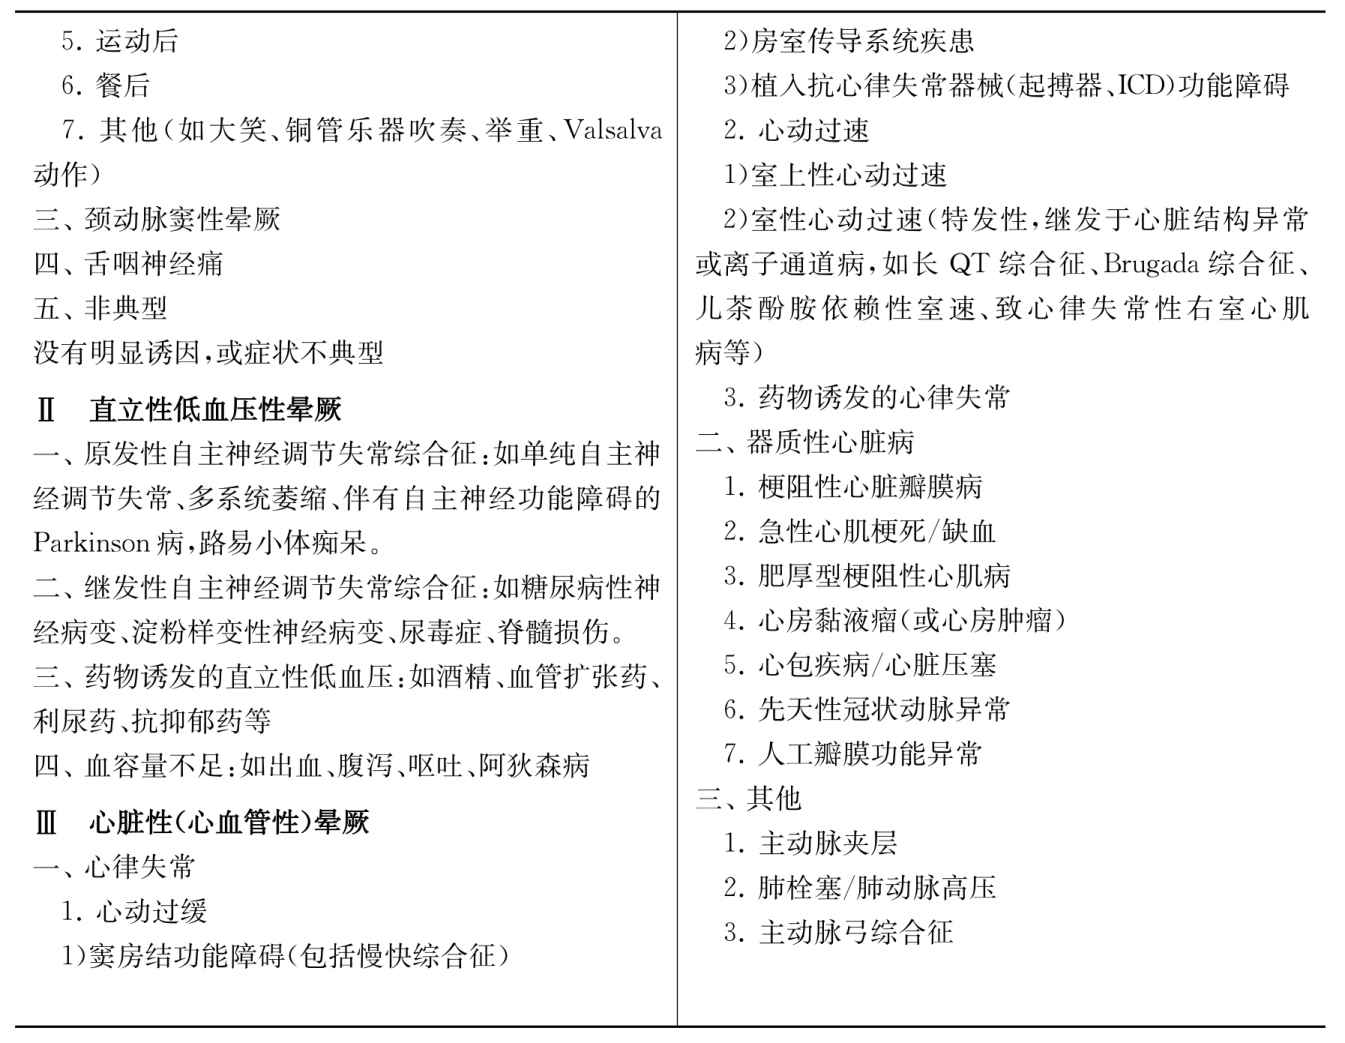
\includegraphics[width=\textwidth,height=\textheight,keepaspectratio]{./images/Image00304.jpg}
 \end{longtable}

\section{【确定是否晕厥】}

\subsection{(一)晕厥的表现}

典型的晕厥发作可分为三期:

\subsubsection{1.晕厥前期}

自主神经症状明显,表现为面色苍白、恶心、出汗、头晕、眩晕、耳鸣、上腹部不适、打哈欠、肢端冷,常有黑蒙,以及轻度肌张力减弱导致患者躯体摇摆。此期持续约几秒至10秒,脑电图表现为脑波频率逐渐减慢以及波幅逐渐增高。部分病例在此期间如能扶持物体或躺下,症状可逐渐消失而不至发生意识丧失。

\subsubsection{2.晕厥期}

意识丧失及肌张力消失,患者可倒地,大多数血压下降,瞳孔散大及对光反射减弱,角膜反射消失,腱反射消失,可有遗尿。脑电图检查见各导联出现慢波,持续整个晕厥期。此期通常为几秒,若意识丧失时间更长,则可发生抽搐。

\subsubsection{3.晕厥后期}

意识恢复,对周围环境能正确理解,仍有面色苍白,全身软弱无力,不愿讲话或活动,或者有恶心、打哈欠、过度换气、心动过缓、头痛,偶有轻度精神紊乱。然而,不少类型的晕厥并无明显的三期表现,却有其独特症状。

\subsection{(二)晕厥的病史询问}

由于医生往往未能目睹患者的晕厥发作,故详细询问病史显得特别重要。病史中尤应注意发作诱因、发作是否突然、发作场合和体位、前驱症状、意识丧失时间有多长、发作的后遗症状、晕厥发生的次数和频繁程度、外伤史、用药史、家族史、神经系统疾病史、心血管病史等。尽可能地了解发作时的伴随症状及体征,特别是面色、血压、脉搏、呼吸、心率及心音的改变,有无伴发抽搐或神经系统局灶体征。

\subsection{(三)确立晕厥的依据}

其依据是发作突然、意识丧失时间短、不能维持正常姿势或倒地、可于短时间内恢复。

\subsection{(四)晕厥的鉴别诊断}

尤其要注意与一些可引起短暂意识障碍的疾病鉴别。

\subsubsection{1.与眩晕的鉴别}

眩晕主要感到自身或周围景物旋转或摇摆晃动的感觉,眼或头部转动时症状增剧,通常无意识障碍。

\subsubsection{2.与昏迷的鉴别}

昏迷的意识障碍持续时间较长,较难恢复,参见第49章。

\subsubsection{3.与休克的鉴别}

休克的早期意识仍清醒,或仅表现为精神迟钝,周围循环衰竭更明显且持久。

\subsubsection{4.与癫痫的鉴别}

癫痫小发作发作无诱因,不倒地,面色、血压及脉搏无改变,发作及终止均比晕厥快,发作完毕可立即继续原来的工作或活动;而晕厥发作后全身软弱无力,不愿讲话或活动,晕厥发作时脉搏减慢、血压下降,脑电图出现普遍性慢波,而癫痫小发作的脑电图见有3Hz的棘慢波。晕厥如伴发抽搐,需与癫痫全面性发作鉴别,后者发作时面色发绀,血压及脉搏改变不明显,抽搐多表现为四肢开始时为强直性继而为痉挛性,而晕厥持续时间较长出现的抽搐多表现为肢体不规则的零星抽动。

\subsubsection{5.与其他原因造成的短暂性意识障碍鉴别}

各种原因造成的代谢紊乱如:低血糖、低氧血症、过度通气造成的低碳酸血症等造成的意识障碍均不属于晕厥;各种原因的中毒和椎基底动脉TIA也需与晕厥鉴别。

\section{【晕厥病因鉴别诊断的相关检查】}

\subsection{(一)与心脏相关的检查}

按需要选择如心电图、超声心动图、心电监测、动态心电图、心脏负荷试验、运动试验,另一方面,如果心脏有异常发现,应进行血流动力学检查和(或)心血管造影方面的评价,以明确其功能上的意义。此外,由于心律失常是器质性心脏病患者发生晕厥最常见的病因,所以应通过无创性检查和创伤性电生理检查来评估患者对快速或缓慢性心律失常的易感性。

\subsection{(二)其他检查}

脑电图、视频脑电图、颈椎X线照片或颈椎CT(或)MRI、脑部CT、MRI、CTA、MRA、脑脊液检测、血管造影等。如果通过初步检查除外了器质性心脏病,倾斜试验则是首选的最有意义的诊断性试验,因为在这种情况下,血管迷走性晕厥的可能性最大。有充分的研究表明,在倾斜角度为60°~70°且没有诱发药物的情况下,倾斜试验的特异性为90\%左右;在有诱发药物的情况下,倾斜试验的特异性降低,但不影响其临床使用。倾斜试验结合创伤性生理检查能提高晕厥病因的诊断率。颈动脉按摩是提示颈动脉窦反射过敏导致晕厥的一种检查方法。

\section{【晕厥鉴别诊断的思路】}

确定为晕厥后,应进一步鉴别是哪一类晕厥并尽可能寻找病因,可按下列线索考虑:

\subsection{(一)发作的诱因及场合}

用力为晕厥发作的诱因者多见于心脏性晕厥,特别是由于心室流出道梗阻性疾病,如主动脉瓣狭窄、原发性肺动脉高压症、梗阻性肥厚型心肌病等,也常见于发绀型先天性心脏病,如Fallot四联症。用力也是引起严重脑血管阻塞的诱因。以疼痛、情绪不稳、恐惧、见血以及长时间站立、或处于拥挤、闷热环境中等为诱因者,多见于血管迷走神经性晕厥。急剧转颈、低头或衣领过紧诱发晕厥者,应想到颈动脉窦性晕厥。从卧位或久蹲位突然转变为直立位时出现的晕厥,最可能是直立性低血压性晕厥。紧接于咳嗽后或吞咽后的晕厥,需考虑为咳嗽性或吞咽性晕厥。在排尿期间或排尿完毕出现的晕厥,大抵是排尿性晕厥。

\subsection{(二)发作的体位}

血管迷走神经性晕厥、颈动脉窦性晕厥(大多数)都在站立或坐位发生,尤其是在拥挤、高温环境下的长时间站立;但心脏性晕厥的发作多与体位无明显关系,可在卧位发生,过度换气综合征也常在卧位发作。直立性低血压性晕厥多在体位变换为直立时,或与有低血压作用药物的使用和剂量改变有密切关系,或在伴有自主神经功能不全的帕金森病叠加,如多系统萎缩等。

\subsection{(三)发作的伴随症状及体征}

面色明显苍白见于神经介导性晕厥,特别是血管迷走神经性晕厥;面色苍白和发绀多为心脏性晕厥。明显的呼吸困难见于心脏性晕厥;呼吸缓慢而带鼾声出现于某些脑源性晕厥。血压显著下降见于直立性低血压晕厥以及血管迷走神经性晕厥,后者尚伴有脉搏缓弱。两上臂收缩压相差大于20mmHg者,要考虑是否有锁骨下动脉盗血综合征或主动脉夹层动脉瘤的可能。心率、心音及心电图改变见于大多数心脏性晕厥,如发现心尖搏动移位、震颤、心脏增大等体征,则更符合心脏性晕厥。颈动脉怒张见于心脏性晕厥,发作后有心前区痛者应怀疑心肌梗死;眼底或周围血管有栓塞,需考虑到心房黏液瘤的可能。

\subsection{(四)过去病史}

心脏性晕厥可存在明确的器质性心脏病,发作之前可有心悸或伴有胸痛,有心脏猝死家族史。神经介导性晕厥可有反复发作的晕厥史。直立性低血压性晕厥者要注意有否帕金森病或帕金森样病病史。

\protect\hypertarget{text00365.html}{}{}

\section{160 神经介导性晕厥}

神经介导性晕厥(neurally mediated syncope,NMS)又称反射性晕厥(reflex
syncope),是指自主神经性心血管功能突然衰竭,引起脑灌注不足所致的一过性意识丧失。NMS的血压下降是急发的、自限性,是压力反射功能一过性损害的结果。由于患者的交感神经活性降低,去甲肾上腺素分泌减少,而肾上腺素、血管紧张素Ⅱ、加压素、内皮素释放增加,激活一氧化氮(NO)合成系统,导致血管扩张和血压下降,其中血管内皮细胞起着重要作用,它能合成具有强烈扩张血管作用的NO。另一方面,当NMS发生时,副交感神经活性增高,乙酰胆碱释放增多,乙酰胆碱能够刺激内皮细胞合成NO。NO扩张血管通过以下机制:①激活腺苷酸环化酶,引起肌浆球蛋白的轻链脱磷酸;②血管平滑肌细胞超极化作用。除晕厥外,NMS患者的自主神经性心血管反射正常,甚至亢进。大多数NMS是由于反射弧的传入通路功能障碍所引起。此外,躯体性疼痛和内脏性疼痛也可成为传入刺激;精神活动也可从大脑皮层经下丘脑传至延髓的心血管运动中枢,故疼痛和情绪不稳均可诱发晕厥。

\subsection{一、血管迷走神经性晕厥(vasovagal syncope,VVS)}

\subsubsection{(一)血管迷走性神经介导的(情感压力)}

也称血管减压性晕厥(vasodepressor syncope)或单纯性晕厥(simple
syncope),是由多种因素触发引起周围血管扩张、低血压和心动过缓所致的自限性晕厥发作。发病主要与交感神经和迷走神经调节反射存在障碍有关,由于外周化学或机械感受器受到刺激,冲动传入延髓的心血管调节中枢,引起神经血管反射,患者从交感神经兴奋突然转为抑制,而迷走神经则过度激活,其传出纤维分别作用于血管和心脏,导致外周血管张力突然降低,引起低血压;由于心脏起搏传导系统受到抑制,引起窦性心律突然骤降,造成大脑缺血、缺氧,从而发生晕厥。VVS通常由非器质性心血管疾病所致,发病率为各类型晕厥之首。本病在男女各年龄段皆可发生,而以年轻体弱女性多见,青少年也是高发年龄段,也有人提出在不明原因晕厥儿童中,VVS的比例大于成人,VVS的发病年龄高峰为5~19岁。另有研究认为儿童晕厥中以VVS最常见。VVS有如下特征:①发作前往往有明显的诱发因素,诱因最常为疼痛、情绪不稳、恐惧、紧张、见血、注射、小手术、天气闷热、拥挤场所、疲劳、久站、饥饿、失眠等;②发作几乎都在站立位或坐位发生,几乎不会在卧位中出现;③发作常常表现为典型的晕厥三期(晕厥前期、晕厥期、晕厥后期),晕厥前期有显著的自主神经失调症状,如面色苍白、出汗、恶心、上腹部不适、眩晕或头晕、耳鸣等,持续数秒至数十秒后进入晕厥期,此期意识丧失,血压速降,脉缓弱(40~50次/分),瞳孔扩大,对光反射迟钝或消失,角膜反射消失,偶尔遗尿。意识丧失时间约几秒至几十秒,可自行苏醒,如让患者平卧,取头低脚高位则恢复较快。晕厥后期症状多数较轻,主要是全身乏力或短期遗忘、精神恍惚。晕厥过后30分钟内不应让患者坐起或站立,否则或可再发。发作时如能检查脑电图,在晕厥期开始可见各导联波幅逐渐变慢并出现对称性2~3Hz慢波,晕厥后期脑波渐恢复正常。不少病例既往有同样的发作或有反射性晕厥的其他类型(如排尿性晕厥)发作。少数病例有家族史。

VVS诊断和鉴别诊断的主要方法是倾斜试验(tilt table
test),在倾斜试验中,以心率减慢为突出表现者为心脏抑制型;以血压下降为突出表现而心率轻度减慢者为血管抑制型;心率和血压均明显下降者为混合型。另一方面,有学者对VVS发作前后进行了Holter监测,结果显示,晕厥前87\%的患者存在无症状心律失常,表现为窦性心动过速、心房颤动;晕厥发作时可出现窦性心动过速,但Holter对VVS的预测效果不如倾斜试验可靠。VVS很少威胁生命,但频繁发作会影响生活质量,也有可能发生意外或外伤。另外有少数患者当晕厥发作时伴有严重的心脏停搏,这是发生猝死的高危人群,故称为恶性VVS。对于那些反复发作、以心脏抑制为主的VVS患者,安装具有频率骤降反应功能的双腔起搏器,可以有效防止晕厥的发作。

本型晕厥的诊断主要根据发作的特点:每次发作都有明显的诱因;在站立位或坐位发生;发作都具有典型晕厥的三期表现;发作时伴有明显的自主神经症状而没有神经系统阳性体征。本型晕厥需注意与某些类型的心源性晕厥相鉴别。

\subsubsection{(二)直立体位介导的(直立位压力)}

如仰卧位低血压综合征,也称为下腔静脉综合征。可发生于妊娠后期的孕妇或腹腔内巨大肿瘤患者取仰卧位时。临床表现主要是血压骤降、心率加快、眩晕、晕厥,这是由于机械性压迫下腔静脉使回心血量骤减所致。如改变为侧卧位或坐位或将肿瘤右移,则症状可缓解。

\subsection{二、情境性晕厥}

情境性晕厥是一种在某些特定情境下出现的晕厥,包括排尿、排便、咳嗽、进食、运动后等行为动作时发生的晕厥,亦属于神经介导性晕厥(反射性晕厥)的一种,因此,情境性晕厥发作时常常存在神经血管反射,迷走神经兴奋,外周血管压力下降,或者存在心率下降,心排血量下降,脑供血不足。不同情境诱发的晕厥患者往往有不同的疾病基础。如排尿性晕厥的患者可有高血压、冠心病、充血性心力衰竭、左室肥厚、十二指肠溃疡、糖尿病等一种或几种疾病,吞咽性晕厥常发生于存在食管痉挛、食管狭窄、松弛,食管癌等食管器质性或功能性病变的患者,咳嗽性晕厥可伴随后颅窝肿瘤、胃食管反流、缩窄性心包炎、慢性阻塞性肺疾病。为何不同情境下均可导致晕厥发作,其中具体机制尚未完全明朗。目前根据血流动力学测定推测大部分情境性晕厥时存在血压下降,导致一过性脑血流供血不足。

\subsubsection{(一)咳嗽性晕厥}

紧接于咳嗽后发生的短暂意识丧失称为咳嗽性晕厥或喉性眩晕(laryngeal
vertigo)。一般认为由于咳嗽时胸腔内压增高而致静脉回流受阻,回心血量减少;同时咳嗽也使颅内压增高,两者均能引起脑血流量减少而发生晕厥。也有人认为可能是胸壁内感受器的一种血管性反射,引起外周血管阻力降低、血压下降而致晕厥。本病多见于慢性支气管炎、哮喘、肺气肿的老年嗜烟患者,或百日咳、支气管哮喘的患儿。发病是在剧烈咳嗽后(有时只咳嗽一声或大笑几声)随即有短暂的意识丧失。部分病例在晕厥前期有短时眩晕、眼花、面色苍白。发作后无不适,不少患者可有反复发作。这种发作偶见于老人用力打喷嚏或用力解便时,也偶见于举重比赛时。

\subsubsection{(二)吞咽性晕厥}

由于舌咽、咽喉、食管和胃的机械性刺激所引起的晕厥,称为吞咽性晕厥(swallowing
syncope)。当吞咽时,沿舌咽神经运动支下行的冲动于颈静脉孔区通过异常传导,经感觉纤维返回脑干,入孤束核并扩散到迷走神经背核而引起晕厥。吞咽性晕厥可见于食管、舌根、咽、喉部或纵隔等部位的疾病,也可见于高度房室传导阻滞、窦性心动过缓、病态窦房结综合征等患者。心肌梗死后由于心脏传导系统对迷走神经兴奋特别敏感,较易发生吞咽性晕厥。晕厥发作与体位无关,但与吞咽食物的性状有关,如硬物、冷、酸、咸、辣等食物易于诱发。饮用含重碳酸钠的饮料,因持续释放CO2时食管内压力增高,易诱发发作。吞咽性晕厥还可见于胆绞痛、胸膜和肺刺激、支气管镜检查时。吞咽性晕厥在发作前、后常无明显不适。

\subsubsection{(三)排尿性晕厥}

发生于排尿时或排尿结束时的晕厥称为排尿性晕厥(micturition
syncope)。发病机制是综合性的:夜间迷走神经张力增高,心率较慢;体位骤变,血液滞留于下肢;排尿时的屏气动作使胸腔内压增高。后两者妨碍静脉回流,是发病的主要因素。另一方面,当胸腔内压增高时静脉压也增加,颅内压也增高,脑血流量减少。而也有人认为与排尿时有Valsalva动作有关,Valsalva动作为紧闭声门时尽力做呼气动作,胸内压力增加,静脉回流减少,心输出量下降,血压下降从而脑血流量减少。患者几乎全为男性,因男性尿道较女性长,排尿时取直立位之故。发病多在20~30岁,也可发生于少年及老年。发作最常在午夜起床排尿时,清晨或午睡起床小便也可发生,天气寒冷或饮酒后较易诱发。晕厥前期症状多不明显,或有极短时的头晕、眼花、下肢发软。患者突然晕倒,意识丧失持续数十秒,自行苏醒。晕厥后期症状通常较轻。本型晕厥的诊断主要根据其发作特点,如以男性患者为主、于排尿过程或排尿后即发生。

\subsubsection{(四)运动后晕厥}

运动后晕厥机制相对可能更清晰一些,其涉及两个相关机制:①运动后过度低血压反应;②神经介导性晕厥,如血管迷走反应,可能前者对后者存在进一步激发作用。运动后低血压反应在步行、跑步、游泳等运动时均可发生,这些患者在运动后常可出现血管扩张,扩张血管的区域不仅包括运动时收缩的肌肉,而且累及未激活的肌肉内血管,动脉血流量升高,继而静脉池的血流量增加,而由于运动后肌肉疲劳,其泵血作用下降,导致静脉内瘀滞血增加,而且运动可导致失水,进一步导致有效循环减少,从而导致回心血量不足,脑血流量下降。虽然心脏前负荷下降可导致心脏代偿性搏动加快,然而这种代偿作用并不足以弥补前者造成的影响。因此目前认为体循环血管阻力持续性下降是运动后晕厥的主要发生机制。另外,运动后肌肉疲劳,肌肉泵血作用下降,且运动时被抑制的迷走神经张力快速恢复,同样导致心输出量下降,这些过程常发生在运动后静止状态的前5~10分钟内。据统计平板试验后神经介导性晕厥的发生率为0.3\%~3\%,但若紧接着进行倾斜试验,晕厥的发生率可增高至50\%~70\%,这说明神经介导作用在运动后晕厥过程中可能并非起严重影响。

综上可以看出,情境性晕厥的发病机制各有特点,不同情境下神经血管反射过程不同,但总的来说基本与自主神经调节功能异常有关,均可导致血压下降或心输出量下降,一过性脑供血不足,共同结局则是造成晕厥。

\subsection{三、颈动脉窦性晕厥}

颈动脉窦性晕厥也称颈动脉窦综合征(carotic sinus
syncope),是由于颈动脉窦反射过敏所致的晕厥。颈动脉窦反射是一种调节血液循环的正常生理反射。正常情况下,兴奋冲动通过神经(主要是舌咽神经第一支即Hering神经)传入延髓,引起迷走神经兴奋,心率减慢;或者引起交感神经的血管抑制纤维兴奋而使血管扩张,血压下降。当颈动脉窦内压力降低时则产生相反的效应。当颈动脉窦或其附近有病变时,颈动脉窦因激惹而反射过敏,可产生发作性眩晕或晕厥。病因最常见是动脉粥样硬化,其他如动脉炎、颈动脉体瘤、近窦处的炎症、肿瘤、淋巴结肿大、瘢痕组织、人为压迫等。发病诱因大多是突然引起颈动脉受压的因素,如急剧转颈、低头、刮面、衣领过紧等。

颈动脉窦性晕厥的特点是:①以中年以上男性多见,青壮年也可罹患;②通常在站立位或坐位发生;③晕厥前期和晕厥后期的症状均不明显;④在意识丧失前可有眩晕,意识丧失时间一般较短,多在数分钟以内,少数病例有抽搐。按其发作时脉搏和血压的改变分为三型:①迷走型:出现晕厥并有明显的窦性心动过缓或房室传导阻滞,偶可发生窦性停搏,本型占70\%;②减压型:出现晕厥伴有血压下降,心率改变不明显。如晕厥伴有心率及血压均明显改变者称混合型;③脑型:因脑血管收缩发生广泛性脑供血不足,出现晕厥,心率及血压变化不大。

颈动脉窦性晕厥的诊断根据上述临床特点,下述两种方法可协助诊断:①颈动脉窦按摩,应在心电图监测下进行,先按摩左侧,需要时再按摩右侧,两侧不能同时进行,每次按摩时间不得超过20秒。颈动脉窦按摩的正常反应是心率减少在5次/分以下,血压下降不超过10mmHg(收缩压)。如出现意识丧失即阳性。颈动脉窦按摩有一定的危险性,还可诱发心搏骤停、脑梗死等,应严格掌握适应证和禁忌证;②发作频繁时以普鲁卡因封闭颈动脉窦,如发作减少也可协助诊断。本病应与血管迷走性晕厥、直立性低血压性晕厥鉴别。

\subsection{四、舌咽神经痛性晕厥}

舌咽神经痛患者在疼痛发作时或紧接发作后,偶尔因迷走神经激惹而发生心率减慢和血压降低,出现晕厥。本类晕厥临床少见,意识丧失时间一般较短,偶或伴有抽搐。触动舌根、扁桃体、耳部等可诱发舌咽神经痛而间接诱发晕厥。

\protect\hypertarget{text00366.html}{}{}

\section{161 直立性低血压性晕厥}

也称体位性低血压(orthostatic
hypotension)晕厥,是从卧位或久蹲位突然转为直立位时发生的一种晕厥,其病因可有:①压力感受器的反射弧受损。反射弧的传入纤维受累,可见于糖尿病、脊髓痨、多发性神经炎;位于脑干网状结构内的血管运动中枢受累,如脑干或颅后窝的急慢性炎症、肿瘤、血管性疾病、外伤等;反射弧的传出纤维受累,见于肌萎缩性侧索硬化、多发性硬化、血卟啉病、脊髓外伤、交感神经切除术后、药物影响(如利血平、胍乙啶、肼屈嗪、氯丙嗪、奋乃静、左旋多巴、司可巴比妥等);②低血容量使心排出量减少。绝对性低血容量可由于大量利尿、失血、失液、肾上腺皮质功能不全所引起;相对性低血容量则可因重度下肢静脉曲张、扩张血管药物所致的血管扩张而引起。缓激肽过高综合征(hyperbradykininism)的患者,由于体内缺乏分解缓激肽的酶,致使血管强烈扩张,患者站立时下肢因静脉和毛细血管高度扩张而呈紫色,静脉回流减少,引起相对性低血容量而发生晕厥。还有一类生理性障碍所致的直立性低血压性晕厥,如长期站立于固定位置(特别是炎热天气,血管更易扩张)、长期卧床、孕妇等,其所发生的晕厥也属于直立性低血压性晕厥。

直立性低血压性晕厥的发生机制是由于正常人从卧位或久蹲位突然改变为直立位时下述三种生理调节发生障碍:①由于地球引力作用,大约300~800ml血液储积于下肢,使回心血量骤减,动脉血压立即下降。这种改变迅即作用于颈动脉窦和主动脉弓的压力感受器,使其发放到血管运动中枢的抑制冲动减少,导致肾上腺能交感神经张力增高,引起心率加速和小动脉收缩,以保证足够的心排出量,因而脑灌注量得以维持,此为最重要的生理调节。②直立位时下肢骨骼肌的肌张力增高和等长收缩,产生“肌肉泵”作用,帮助血液通过静脉瓣流回心脏。③由于体位改变发生过度换气,胸腔内负压增加,有助于心脏充盈。直立性低血压患者乃因从卧位迅速转为直立位时引起血液重新分布,大量血液聚积于下肢,回心血量减少,导致晕厥。当时交感神经活性增高,外周血管收缩,心率加快,但直力性低血压性晕厥与血管迷走性晕厥不同的是前者的迷走神经并未被激活。此外,直立位时心脏向脑供血需克服平均45cm的心脑间距所形成的静脉压(相当于33mmHg),故于直立位时容易发生晕厥。

本型晕厥的主要表现是患者从卧位或久蹲位突然转为直立位的短暂时间内,常常出现头晕、眩晕、眼花、下肢发软,严重者发生晕厥。晕厥的特点是:①通常无诱因;②晕厥前期和晕厥后期的症状均不明显;③意识丧失时间短;④血压急骤下降,心率无大改变(继发于低血容量者可有心动加速);⑤立即卧床则症状可缓解。

诊断根据是晕厥出现的特定场合(从卧位或久蹲位快速起立)、无前驱症状、血压速降、卧床即缓解等特点。疑诊者可作血压体位试验以协助诊断,方法是让患者平卧,2分钟后测量血压,站立后1分钟内测量立位血压。5分钟后按此顺序复测一遍。正常人站立时收缩压下降一般不超过20mmHg,舒张压基本不下降,通过躯体的调节反射于30~40秒内血压回升。如直立位收缩压下降20mmHg以上,舒张压下降大于10mmHg,且持续较长时间不恢复,同时出现脑缺血症状者,可诊断为直立性低血压。本病若为隐性,可在作此试验前嘱患者先做体力活动,引起小动脉扩张则较易诱发。

直立性低血压需与血管迷走性晕厥以及特发性直立性低血压鉴别,血管迷走性晕厥的发病有明显诱因,晕厥的三期症状较典型,发作时除血压速降外心率也明显减慢。特发性直立性低血压除表现为直立性低血压性晕厥外,还有多种自主神经功能损害的表现。

\subsection{一、原发性自主神经调节失常综合征}

\subsubsection{(一)单纯自主神经调节失常}

既往将此型归类为特发性直立性低血压周围型,又称为纯自主神经损害(pure
autonomic failure),由Bradbury和Eggleston于1925年描述,故也称为Bradbury
Eggleston综合征。其病理改变主要累及节后交感神经元,神经细胞变性、丢失;副交感神经损害,中枢神经系统不受累。生化改变主要是在卧位时血中去甲肾上腺素水平降低。部分患者也可发展为多系统萎缩。

\subsubsection{(二)多系统萎缩(multiple system atrophy.MSA)}

多系统萎缩是一神经变性疾病,临床表现为自主神经功能障碍,并且常伴有不典型帕金森病症状、共济失调或锥体束征等。既往将以自主神经功能障碍为突出症状的称为特发性直立性低血压(中枢型)、原发性直立性低血压、特发性自主神经功能不全(idiopathic
autonomic
insufficiency),属于多系统萎缩(MSA)三个亚型中的一个亚型,亦称为Shy-Drager综合征(Shy和Drager于1960年和1961年分别详述。有学者不主张用此名称,也不同意其为MSA的一种亚型)。目前认为MSA包括自主神经功能障碍伴左旋多巴非敏感性帕金森症状(MSA-P亚型)、伴小脑性共济失调(MSA-C亚型)、或三种症状共存。

病理学特征改变为少突胶质细胞的α-突触核蛋白(alpha-synuclein,AS)包涵体。病变部位早期主要在胸腰髓侧角的交感神经元,其后(也可能同时)脑干及骶髓的副交感神经元也累及,位于第1和第2骶节的前角灰质柱中的Onuf核受损,Onuf核是支配会阴横纹肌的脊髓低级中枢,发出的纤维支配骨盆底部肌肉和肛门以及尿道括约肌。随着疾病的进展,纹状体黑质系统、橄榄脑桥小脑系统也有同样的损害,程度较轻。病理改变特征是神经元细胞丧失、星形胶质细胞增生、少突胶质细胞胞浆内有包涵体。生化改变主要是在卧位时血中去甲肾上腺素水平正常或升高(与周围型相反)。

本型晕厥在中年以上男性多见(男∶女=5∶1),隐袭起病,缓慢发展,首发症状可以是交感神经或副交感神经系损害症状,交感神经系的突出症状是位置性低血压,平卧位转为直立位时收缩压下降20mmHg以上,舒张压下降10mmHg以上。患者感到全身无力、头晕、眩晕、黑蒙甚至晕厥;副交感神经系统的突出表现是泌尿和性功能障碍,如尿失禁或潴留;便秘或腹泻;性功能障碍、阳痿;出汗异常、体表温度异常,瞳孔不等大。交感和副交感损害可同时或不一定同时出现。疾病逐渐发展时,锥体外系、小脑、锥体系等运动损害几乎不能幸免。

自主神经系统病损的表现有:①在交感神经功能障碍中,因肾上腺能不足造成的最常见的症状是位置性低血压、射精不能,因胆碱能不足造成的常见症状是无汗。②副交感神经功能障碍的表现有:固定心率、尿潴留、尿失禁、便秘和阳痿等。喉鸣(吸气喘鸣)、呼吸暂停和呼吸困难,严重时需气管切开,这是因为延髓的疑核萎缩造成声带外展麻痹所致;也可能是由于喉肌的肌张力不全或运动障碍,或者是两种因素均存在。喉鸣的出现对本综合征的诊断颇有价值。呼吸困难还可能是延髓腹外侧的NK-1R-LI神经元(neurokinin-1receptor-lik-\/-immunoreactive
neurons,NK-1R-LI)严重损害所致。吞咽障碍也可能是多系统病损所引起。此外,患者还有中枢性和梗阻性呼吸暂停、睡眠障碍、吞咽障碍。患者于卧位时去甲肾上腺素水平正常或升高,血压正常甚至增高(本型患者除了低血压以外也可发生高血压,特别是夜间由于高血压导致脑出血死亡);少数患者由于夜间迷走神经功能亢进,可发生心搏骤停而猝死。

MSP的诊断和鉴别诊断比较困难且有争议,在疾病早期如果只有自主神经功能障碍而多系统症状尚未出现,则其诊断不能确定。此后陆续出现帕金森综合征、小脑损害及锥体系统症状时,诊断才得以明朗。辅助检查可作体位性血压测定以协助诊断,在作此检查时除可发现血压因体位直立而降低外,不少患者同时出现眩晕、黑蒙,偶尔晕厥。脑CT检查可见小脑萎缩,MRI平扫可见壳核、小脑中脚和脑桥萎缩,黑质致密带和壳核后外侧有低信号(是否铁沉积未能确定),其中T2加权相中“十字征”和“裂隙征”是MSA的特征性但非特异性改变,这些特征均可作为诊断的参考。

MSP的鉴别诊断很重要,以小脑损害症状突出者,主要表现为步态不稳、肢体共济失调、眼球震颤、小脑性构音障碍,需与散发性脊髓小脑性共济失调鉴别。后者多为常染色体显性遗传,进展较慢,常有阳性家族史,无明显自主神经功能症状。以帕金森综合征表现为主者,主要表现为肢体震颤、肌强直、动作缓慢,需与帕金森病鉴别,MSA对左旋多巴的反应不佳或仅有轻微疗效,自主神经功能障碍出现早并且严重有助鉴别。另外,临床鉴别有困难者,可借助一些辅助检查,如:容积系列MRI,18氟-荧光脱氧葡萄糖PET结合多巴胺转运体PET,肛门括约肌肌电图等,对鉴别诊断有一定帮助。另外,当疾病早期,其他神经系统症状体征不明显时,尚需与非神经源性直立性低血压鉴别,后者当体位改变引起晕厥时可伴心率增快;也需与糖尿病性周围神经病、淀粉样变性病所引起的继发性自主神经损害鉴别,这两种慢性变性疾病的自主神经功能障碍都很明显,但均有周围神经系病损以及原发病可寻。本综合征预后不佳,患者发病后一般于7~10年死亡。

\subsubsection{(三)伴有自主神经功能障碍的帕金森病}

帕金森病患者较普遍地伴有自主神经功能障碍,如皮脂溢、多汗、直立性低血压、流涎、便秘、尿失禁、性功能障碍等,这与帕金森病变所累及的范围较广泛有关,除累及黑质、蓝斑外,其他部位如下丘脑背部、迷走神经背核、交感神经节、肾上腺髓质也受影响。蓝斑、下丘脑背部、迷走神经背核为多巴胺能神经元,这些部位的损害可造成自主神经功能障碍,尤其与直立性低血压有关,患者可有乏力感、头晕、黑蒙甚至晕厥,据现有文献可能有约20\%~50\%的帕金森病患者伴有直立性低血压,在年龄较大、病程较长的患者中更多见,但也有报道在疾病早期,甚至在帕金森典型症状出现前便可出现直立性低血压症状,然而这也需要与多系统萎缩进行鉴别。帕金森病患者血浆儿茶酚胺含量较正常人降低,直立位时血浆去甲肾上腺素增幅小,有些帕金森病患者虽然在一般状态下,上述物质在正常范围,但在下丘脑-垂体-肾上腺轴受到刺激时,ACTH和儿茶酚胺上调速度明显减缓。帕金森病伴有直立性低血压患者在立位时,心脏迷走神经增强反射和血浆去甲肾上腺素增加量均明显降低,且因自主神经功能损害,骨骼肌和内脏血管的感受压力变化及通过交感调节收缩的功能下降,外周阻力血管呈现去交感支配的倾向,这些都可导致直立性低血压表现。

帕金森治疗药物也可产生心血管系统的副作用,合并用药较单用左旋多巴有更高的心电图异常、心血管反射减弱及体位性低血压,抗胆碱药、溴隐亭等多巴胺受体激动剂与脱羧酶抑制剂的合剂等也被认为是直立性低血压的原因。儿茶酚氧位甲基转移酶抑制剂(恩他卡朋)可以轻度收缩血管而产生升高血压的作用,提示与左旋多巴合用可减少直立性低血压的发生率。

帕金森病和帕金森综合征常常难以鉴别,而对自主神经系统的评价有助于两者鉴别。便秘于帕金森病发病早期多见,其余多数自主神经症状特别是心血管系统的症状在发病初期一般不出现,即使出现也很轻,因此出现较明显的心血管系统自主神经障碍时,应考虑帕金森病以外的疾病。而对左旋多巴反应良好又表现为广泛明显的自主神经障碍的患者,亦更支持帕金森病伴自主神经障碍。帕金森病自主神经病变以节后神经病变为主,而MSA神经节或节前病变更常见,这也是一个鉴别点。

\subsubsection{(四)路易小体痴呆(dementia with Lewy bodies,DLB)}

路易小体痴呆是一种神经系统变性疾病,其主要临床表现为波动性认知障碍、帕金森综合征及以视幻觉为突出代表的精神症状。1961年Okazaki等首次描述该病。主要的病理表现为皮层和皮层下有大量的Lewy小体。

临床表现有:进行性、波动性的认知功能障碍,可在正常和异常间波动,同时伴有觉醒状态和注意力的波动;精神症状表现为视幻觉(80\%),谵妄,异常行为,抑郁;帕金森综合征表现为僵硬、动作迟缓多见,一般较轻微,四肢多对称出现,震颤少见,左旋多巴疗效欠佳。此外,还可见自主神经症状(体位性低血压、尿失禁),反复跌倒,晕厥,短暂意识丧失,快速眼动期睡眠障碍。对常规剂量的神经安定药物出现严重的副作用。头颅CT、MRI正常或轻度弥漫性脑萎缩,与AD相比,颞叶内侧萎缩程度轻者高度提示DLB。PET显示颞顶枕皮质的低代谢,枕部代谢减低远远重于AD。

诊断根据下列三项特征中存在两项可拟诊DLB,一项为可疑DLB:①波动性认知障碍,以注意和警觉障碍波动尤为明显;②反复发作形式完整、内容具体的视幻觉;③自发性帕金森综合征的运动特征。鉴别诊断上需与血管性痴呆,克雅病(Creutzfeldt-Jakob
disease,CJD),进行性核上性眼肌麻痹(PSP),药物中毒等鉴别。血管性痴呆多有反复卒中病史,突然起病,阶梯样进展,有局灶神经系统症状和体征,无明显的视幻觉,头颅CT或MRI可见多发的梗死灶。克雅病主要表现快速进行性痴呆,可有视力障碍和视幻觉,肌阵挛,早期头颅MRI的
DWI成像可见皮质异常信号,呈彩带样改变,脑脊液蛋白阳性,脑电图具有典型的周期发放的高幅棘-慢综合波(PSWC),进展快,病程多为1年。进行性核上性眼肌麻痹在眼球运动障碍出现之前,较难鉴别,但PSP的痴呆无症状波动,视幻觉少见。老年患者要注意有否药物因素引起,注意询问用药情况,如为药物作用所致视幻觉、体位性低血压、认知功能改变等,在停药后症状可缓解。

\subsection{二、继发性自主神经调节失常综合征}

\subsubsection{(一)糖尿病性自主神经病变导致的晕厥}

约有20\%~40\%的糖尿病患者(diabetic autonomic
neuropathy,DAN)合并有自主神经病变,尤其是心血管自主神经病变。在糖尿病早期甚至在糖尿病症状及体征出现之前,患者已可有心血管及其他系统的自主神经功能异常,但由于起病隐匿,且长时间无临床症状,容易被患者和医师忽视,然而糖尿病性心血管自主神经病变后果严重,与糖尿病患者无症状性心肌缺血和无痛性心肌梗死有关,需高度重视并及时干预。

糖尿病性自主神经病变的病理机制尚不清楚,相关的假说包括:①高血糖引起一系列的代谢障碍影响神经系统;②微血管病变引起神经缺血;③自身免疫性损害;④神经生长因子缺乏。体位性低血压是DAN的常见表现,通常认为,糖尿病患者自主神经先表现为副交感神经病变,而体位性低血压则为晚期的交感神经病变表现,是由于交感神经传出纤维受损,特别是支配内脏血管的纤维受损,皮肤、内脏及全身血管阻力下降也容易导致体位性低血压。一般情况下,体位改变时血浆去甲肾上腺素增加以调节血管收缩活动,在糖尿病性体位性低血压患者这种反应减弱,出现血压下降。心脏收缩功能减弱也参与了体位性低血压的发生。

DAN导致的体位性低血压可表现为乏力、疲劳、头晕、心慌甚至晕厥等症状,但有些患者在血压明显下降时也没有明显症状,对于这些患者需进行教育,避免容易出现低血压的行为和环境,如避免起床过快,避免热水淋浴。少数患者还同时可合并卧位高血压,因此对于这些患者不仅要控制体位性低血压,还需防止卧位高血压的发生,如睡前限水,避免夜间使用控制低血压药物米多君等。

\subsubsection{(二)淀粉样变性周围神经病相关的自主神经损害}

淀粉样变性周围神经病指的是淀粉样物质在周围神经沉积,引起的一组严重的进行性感觉、运动周围神经病,伴自主神经功能障碍,主要包括家族性淀粉样变性周围神经病、原发性轻链淀粉样变性、透析相关/β2微球蛋白淀粉样变性等。所谓淀粉样物质是生理状态下可溶性蛋白质在一些病理因子作用下形成β折叠结构,使其变为不可溶的蛋白质并在多个器官或组织的细胞外沉积,这些蛋白包括:转甲蛋白,主要见于家族性淀粉样变性周围神经病;免疫球蛋白的轻链(κ链和λ链),由浆细胞产生,见于原发性轻链淀粉样变性和浆细胞增生症;β-微球蛋白,见于肾衰后长期透析的患者;另外还有糖尿病相关胰岛淀粉样多肽链、载脂蛋白系列、血清淀粉样物质A和胶质蛋白等。

其中家族性淀粉样变性周围神经病(hereditary amyloid
neuropathy,HAN),是常染色显性遗传病,主要损害感觉、运动和自主神经,常伴有内脏损害。HAN是由于基因突变导致血浆中不可溶的纤维状蛋白发生β折叠,进一步沉积形成淀粉样物而致。研究已发现该病可分别由ATTR、ApoA1或Gelsolin基因的缺陷所引起。其中ATTR基因突变最为多见。HAN患者最容易累及周围神经,往往在疾病早期即出现自主神经纤维受损,主要累及心血管、胃肠道、泌尿生殖等系统。心血管系统自主神经异常可导致体位性低血压,可无症状,或站立时出现疲乏、黑蒙、头晕,胃肠道自主神经损害可导致餐后腹泻和餐后呕吐症状,可引起脱水,进一步加重体位性低血压症状。淀粉样蛋白沉积还可累及心脏传导系统、心肌细胞,出现心律失常、束支传导阻滞、限制性心脏病,可出现头晕、晕厥,甚至猝死。对于这一类患者应及早进行血压监测及心电生理检查、心脏彩超评估心功能,评估其危险性,及早进行干预。增加摄入盐引起适当水钠潴留,穿弹力袜,少食多餐、胃动力和止呕药可改善呕吐症状,阿片类药物、奥曲肽减轻腹泻,及时补液纠正脱水,口服盐酸米多君收缩小静脉和小动脉,增加外周阻力,均有助于改善体位性低血压。

\subsection{三、药物诱发的直立性低血压}

临床上常见应用药物后引起动脉血压降至90/60mmHg以下,患者可伴有头晕、乏力、精神不振,甚至出现晕厥等临床症状,称为药源性低血压。某些高血压患者使用某种药物后出现血压下降过快或下降幅度过大,同时出现低血压的临床表现,即使动脉血压并未降至90/
60mmHg时也视为药源性低血压。治疗心血管疾病的药物是临床最常见的致低血压药物,包括抗心绞痛药物、α肾上腺素受体阻滞药物、钙离子拮抗剂、β受体阻滞剂、血管紧张素转换酶抑制剂、血管紧张素Ⅱ受体拮抗剂、利尿剂等均可导致低血压,另外丹参、灯盏花素、地巴唑等具有血管扩张作用的药物也可导致低血压反应。中枢神经和周围神经相关药物导致的低血压也很常见,包括抗精神病药如氯丙嗪、奥氮平等,抗抑郁药物阿米替林等,抗震颤麻痹药物、麻醉、镇静镇痛、催眠药物亦可导致血压下降,抗生素包括青霉素类、部分头孢类、氨基糖苷类、喹诺酮类药物可导致低血压,急剧降低血容量、引起过敏反应的药物、酒精也易引起低血压。另外消化系统药物、抗过敏药物导致的低血压也见诸报道。

药源性低血压的机制包括:①血管扩张作用,大多数药物可直接或间接扩张血管导致低血压,降血压药物通过不同机制扩张血管,抗精神病性药物所致体位性低血压与抑制中枢调节的加压反射和阻滞外周α肾上腺素受体有关,麻醉镇静药、肌松药、导致过敏的药物等可通过释放组胺引起血管扩张、通透性增高,饮酒后体内乙醛堆积产生戒酒硫样反应,可导致血压下降;②心肌收缩力的抑制作用:胺碘酮、普萘洛尔等抗心律失常药物通过抑制心肌收缩力、减慢心率而使心排血量减少,动脉血管充盈不足引起血压下降;③血容量减少:呋塞米、甘露醇可导致利尿,解热镇痛药通过发汗导致有效血容量下降,血压降低;④神经节阻滞和促进介质释放:溴丙胺太林、美卡拉明等具有神经节阻滞作用,利血平则可耗竭交感神经末梢儿茶酚胺而使交感神经张力下降,外周小动脉扩张;⑤不良的药物相互作用:不同降压药合用是可出现降血压的相加作用导致血压过低,氯丙嗪、多巴胺与α肾上腺素受体阻滞药物合用的降压作用剧烈,应当避免联合用药。

当患者服药治疗期间血压降至90/60mmHg以下,或高血压患者用药后血压明显降低,并出现头昏、眩晕、乏力、嗜睡甚至晕厥等症状时,需高度怀疑药源性低血压。当患者卧位血压正常,而从卧位突然变成坐位或立位时收缩压下降20mmHg以上,舒张压下降大于10mmHg,应怀疑存在药源性体位性低血压。这时需仔细询问用药史,明确药物使用与低血压症状的因果关系,并排除脑血管病、低血糖、癫痫等其他原因所致情况。对于药源性低血压患者,可调整药物剂量,严重低血压者需立即停药,补充血容量或使用升压药。明确导致低血压的药物后,使用上述对策升压不明显时可使用特异拮抗剂治疗。

\subsection{四、血容量不足}

各种原因如大量失血,频繁的腹泻、呕吐,阿狄森病等导致的血容量不足,均可引起头昏、眩晕、乏力,甚至晕厥。阿狄森病(Addison
disease)又称原发性肾上腺功能不足(primary adrenal
insufficiency),由于肾上腺无法分泌足够的皮质醇,血中皮质醇浓度降低,导致血钠降低,血容量降低,引起体位性低血压。此外,尚有轻度倦怠感、无精神、皮肤颜色变黑、易怒、体重减轻、四肢肌力下降、恶心、呕吐等,症状于运动后恶化,卧床休息后好转。实验室检查发现血糖下降,血钾升高,ACTH兴奋试验反应低于正常水平,B超或CT提示肾上腺萎缩或增大、破坏、钙化。

\protect\hypertarget{text00367.html}{}{}

\section{162 心脏性晕厥}

心脏性晕厥(cardiac
syncope)占全部晕厥的9\%~34\%。引起心脏性晕厥的情况有:心搏停止;心律失常(心动过速或过缓);心室流入道或流出道受阻;心内由右至左分流增加;渗漏或裂解的主动脉瘤;急性肺动脉栓塞等。表\ref{tab48-1}中所列的心脏疾病均可引起心脏性晕厥。由于神经介导性(或称神经反射性)心搏减慢或停止所致的晕厥,本章将之归入神经介导性晕厥范畴(见上文)。心脏性晕厥的发生是由于急性心搏出量骤减,随即脑灌注量急降而出现晕厥,晕厥可发生于卧位、体力活动时或活动后。心脏性晕厥在各类晕厥中最危险,猝死常见于心脏性晕厥,大多数晕厥患者的猝死原因为心律失常。

\subsection{一、心律失常所致的晕厥}

在心脏性晕厥中,以心律失常所致的晕厥最常见。由于各种疾病或药物的毒性作用,引起心脏停搏、心动过缓(低于35~40次/分)、室性心动过速或心室颤动,使心排出量剧减或中断,导致脑灌注压低而发生晕厥。最多见于不完全性房室传导阻滞突然转变为完全性房室传导阻滞时,其他如高度房室传导阻滞、慢性双分支阻滞、室性或室上性阵发性心动过速、心室颤动等。任何原因导致的心脏停搏若持续3~5秒(直立位)或15秒(卧位)往往发生晕厥,如脑灌注压继续低则可发生抽搐样动作,也可有大、小便失禁。

\subsubsection{(一)病态窦房结综合征}

开始常表现为头晕、眼花,逐渐加重后可出现晕厥。大约40\%~80\%的患者会发生晕厥。晕厥通常在窦性停搏、严重心动过缓等情况下发生。病态窦房结综合征所致的晕厥有时需与血管迷走性晕厥鉴别,倾斜试验阳性支持后者的诊断。

\subsubsection{(二)二尖瓣脱垂}

又称click
murmur综合征,是一种常见的、伴发室上性或室性心律失常的疾病。女性患者两倍于男性患者。在一组病例统计中,25\%的患者诉头晕或眩晕,而4\%发生晕厥。最常见的主诉是一种有特征性的非用力性的不典型胸痛,多为左胸口的尖锐痛,持续时间长短不等,随之是呼吸困难和疲倦。还可出现重度室性心律失常以及极度心率缓慢。心脏听诊可闻及收缩中期咔嗒音。心电图可以完全正常或出现非特异性ST-T波改变。频发性室性期前收缩常见。本病可借超声心动图诊断。

\subsubsection{(三)遗传性Q-T间期延长综合征}

遗传性Q-T间期延长综合征(hereditary long Q-T interval
syndrome,LQT)以反复发作的晕厥、抽搐为特征,心电图显示Q-T间期延长、尖端扭转型室性心动过速或心室颤动。本综合征又分为三个亚型:

1.Ⅰ型:Jerrell Large
Nielson综合征,伴有先天性耳聋,又称聋-心综合征(surdo-cardiac
syndrome),常染色体隐性遗传。特点是先天性神经性耳聋、心律失常、发作性晕厥、猝死,心电图显示Q-T间期延长、尖端扭转型室性心动过速或心室颤动。

2.Ⅱ型:Romano Ward综合征,无耳聋,常染色体显性遗传。

3.Ⅲ型:又称低钾性遗传性LQT,无耳聋,伴有血清钾低。LQTS是由于编码心肌细胞膜钾或钠离子通道的基因突变引起的、具有相同表型的一组疾病,现已发现7个基因突变与本综合征有关,据此分为7个亚型,其中以LQT1型的发病率最高,占42\%,它是由11p15.5上的KCNQ1基因突变所致。梁璐等在6个家系13例患儿的基因检测中发现KCNQ1基因的2个新缺失突变位点和1个新的多态位点,分别来自6个家系中的2个家系。Q-T间期延长综合征的初次发作多在幼年,10岁前发病最多。临床主要表现为晕厥,发作诱因常为焦虑、恐惧、疲劳、突然的巨大声响。发作前某些患者可有先兆,如胸闷、心悸、黑蒙、嗅觉异常或(及)似有风吹过面部或躯体的感觉。意识丧失时间持续数秒至数十分钟,最长一天,间可伴有抽搐及尿失禁,面色开始时苍白,继而发绀。发作后数分钟内定向障碍、恶心、呕吐、头痛、全身不适、嗜睡。神经系统及脑电图检查多无异常,心电图检查可见T波宽大、平坦、高尖,常见U波,不同程度的Q-T(或Q-U)间期延长是本综合征的心电图特征性改变。晕厥发作时出现各种快速型室性心律失常。LQT的诊断标准:反复发作的晕厥,首次发作多在20岁前;Q-T间期延长伴QU或TU畸形;发作时有短暂室颤、室速。本综合征需与癫痫大发作鉴别,后者发作时脉搏和心率无明显改变,肢体先有强直性继而阵挛性抽搐,发作全过程仅为几分钟,面色开始即为发绀。心电图改变有助于这两种病的鉴别。还需与癔症、获得性Q-T间期延长、家族性室颤综合征鉴别。LQT患者约40\%的病例最终发生猝死,2/3的死亡病例在10岁以前。

\subsubsection{(四)药物中毒所致的心源性晕厥}

奎尼丁可引起室性心动过速、心室颤动或心脏停搏而导致晕厥,称为奎尼丁晕厥(quinidine
syncope)。引起发作的因素有充血性心力衰竭、并用洋地黄、肝功能障碍、高或低血钾、电击除颤损伤等。心室颤动所致的奎尼丁晕厥,是使用奎尼丁引起猝死最主要和最常见的原因。奎尼丁晕厥可发生在患者全无奎尼丁中毒症状的情况下,使用小剂量或血浆浓度低于有效水平时也可发生晕厥。晕厥的特点是通常无先兆,发作突然。意识丧失,伴有明显苍白或兼有发绀,持续30秒至3分钟左右,多可自然终止。常有复发,甚至使用小剂量奎尼丁也可复发。约半数患者在发作前无心电图改变,但连续描记也可发现一些引起晕厥的预兆,如各种过早搏动、各种程度的传导阻滞、Q-T间期延长和(或)明显的U波。其他可致心源性晕厥的药物还有洋地黄、酒石酸锑钾、普鲁卡因胺、普萘洛尔、吩噻嗪类、三环类抗郁药等。

\subsection{二、左心房黏液瘤与左心房巨大血栓}

左心房黏液瘤可发生在任何年龄,绝大多数发病于30~60岁,女性受累三倍于男性,发病可能与遗传有关。左心房黏液瘤与左心房巨大血栓可产生左室流入或流出道梗阻,导致心搏出量骤减,引起晕厥。可伴呼吸困难、充血性心力衰竭、二尖瓣区杂音、发热、瘀斑、血沉增快、左房室瓣回流。超声心动图检查是诊断黏液瘤的可靠方法。此外,细菌性心内膜炎的赘生物、人工瓣膜功能不良也可引起机械性阻塞,而发生晕厥。

\subsection{三、限制性心包炎或心包填塞}

在这两种情况下,任何位置的移动或减慢心率或减少静脉回流的药物,都可能引起突然的心排出量不足而导致晕厥。

\subsection{四、主动脉瓣狭窄}

约有10\%的主动脉瓣狭窄病例(先天性或获得性,各年龄组均有)发生晕厥,乃由于左心室流出道梗阻、心排出量减少所致。几乎所有的患者在晕厥前都有用力史。部分病例有短暂的前驱症状如头晕、眼花、出冷汗,或有短促呼吸和心绞痛。晕厥时间可长可短,可伴有心律失常及抽搐。体检可发现特征性收缩期杂音(常伴有可触到的颤动)。这些患者35岁后作影像学检查可发现瓣膜钙化,超声心动图检查可确诊。晕厥发作后一般预后不佳,如无治疗则存活时间平均为18个月至3年,故确诊后应速行瓣膜置换术。

\subsection{五、梗阻性肥厚型心肌病}

梗阻性肥厚型心肌病的梗阻型也称“特发性肥厚型主动脉瓣下狭窄”,包括一组常染色体显性遗传伴有不同遗传度的心肌病。最常见的主诉是呼吸困难(60\%),晕厥次之(30\%),胸痛也是常见症状。晕厥常于20~30岁出现,晕厥的特征是发生在运动时或运动后,也可发生在直立时或咳嗽后。可由于左心室流出道受阻,左心室顺应性减低而充盈欠佳;或发生快速心律失常,导致脑缺血所致。王燕等对一组85例肥厚型心肌病患者的研究分析中,发现有晕厥或黑蒙者24例,占28.2\%,还发现缓慢型心律失常组21例中,有1例合并轻度左心室流出道梗阻,有晕厥发作史;而快速型心律失常组30例中,有3例合并左心室流出道梗阻,均有晕厥发作史。此外,限制型原发性心肌病可引起左心室流入道梗阻而发生晕厥。

\subsection{六、心肌梗死}

心肌梗死引起的晕厥以发生在左心室前壁梗死者居多,因左心室前壁内神经丛与颈动脉窦有联系。急性心肌梗死以晕厥为主要表现者,多见于伴有高血压或老年冠心病者,发病可有两种情况:①晕厥发作时听不到心音或有心律失常,发作后方出现心前区疼痛,也可没有心前区疼痛,需作心电图描记始能及时确诊为心肌梗死;②出现明显的心前区疼痛后才发生晕厥。急性心肌梗死所致的晕厥其持续时间较长,偶有尿失禁,抽搐少见,意识恢复后某些患者有恶心、呕吐、全身无力。

\subsection{七、先天性心脏病}

先天性心脏病合并右至左分流者发生晕厥比其他类型的先天性心脏病常见,其中以法洛(Fallot)四联症引起者居多,患儿在啼哭或用力时,由于外周血管的阻力下降,使由右向左的分流增加,动脉血氧饱和度降低而致晕厥。刘芳等对一组“儿童晕厥30例病因分析”的研究中,3例为法洛四联症,均为哭吵后发生晕厥,其中2例反复晕厥并伴有抽搐,3例都有明显发绀和心脏杂音,心导管检查证实右室流出道均严重狭窄。

\subsection{八、肺动脉高压症和肺动脉血栓}

肺动脉高压症患者在用力时或用力后发生晕厥,其原因主要是心肌缺血,导致心室颤动、心排出量剧减所致。晕厥前有短时头晕、眼花、上腹部不适、窒息感以及心脏紧迫感、用力性呼吸困难,意识丧失常伴发绀。本病若发生晕厥可能是猝死的先兆。血气分析即使安静状态也呈低氧血症。另外,在巨大的肺动脉栓塞患者中20\%可发生晕厥(但微细的肺动脉栓塞则是晕厥的少见原因),晕厥消失后,患者往往诉胸痛、呼吸困难、恐惧。检查可见低血压、心率快、呼吸急速,明显的动脉低氧血症。

\subsection{九、夹层主动脉瘤}

大约5\%~10\%的急性主动脉裂解(acute aortic
dissection)可发生孤立性晕厥,其他神经症状可出现或不出现。主动脉裂解患者中约15\%是无痛的。综上所述,心源性晕厥的特点是:发作与体位一般无关;用力常为发作诱因(所谓用力性晕厥);前驱症状多不明显,或有心悸、胸痛;主要伴随症状是面色苍白合并发绀、呼吸困难、颈静脉怒张、心率、心音和脉搏改变;心电图多有异常;患者常有心脏病史或(及)心脏病体征。

\subsection{十、主动脉弓综合征(无脉病)}

是一种大血管的全动脉炎,亚洲妇女最常见。约有35\%~75\%的患者发生晕厥,患者可在起立、走路或活动过剧时,由于减少了到脑部的血流量而发生晕厥,特别是在运动后、站立或头部活动时。体检可发现双侧动脉搏动减弱或消失,两侧血压降低。

\protect\hypertarget{text00368.html}{}{}

\section{参考文献}

1.The Task Force for the Diagnosis and Management of Syncope,et
al.Guidelines for the diagnosis and management of syncope(version
2009).European Heart Journal,2009,30(21):2631-2671

2.刘志刚,等.心脏起搏防治血管迷走性晕厥的研究.中华心血管病杂志,2005,33(1):3330-3332

3.刘芳,等.儿童晕厥30例病因及临床资料分析.中国实用儿科杂志,2004,19(11):660-662

4.吕家高,等.268名不明原因晕厥患者电生理检查结果分析.中华心律失常学杂志,2003,7(2):115-116

5.张清友,杜军保,李万镇.舌下含化硝酸甘油直立倾斜试验对儿童不明原因晕厥的诊断研究.中华儿科杂志,2004,42(5):37371-37458

6.中华心血管病杂志编委会倾斜试验对策专题组.倾斜试验用于诊断血管迷走性晕厥的建议.中华心血管病杂志,1998,26(5)∶325-327

7.Livanis EG,et al.Situational syncope:response to head-up tilt
testing and follow-up:comparison with vasovagal syncope.Pacing Clin
Electrophysiol,2004,27(7):918-923

8.Kakuchi H,Sato N,Kawamura Y.Swallow syncope associated with complete
atrioventricular block and vasovagal
syncope.Heart,2000,83(6):702-704

9.Krediet CT,et al.Exercise related syncope,when it's not the
heart.Clin Auton Res,2004,14Suppl 1:25-36

10.Freeman R,et al.Consensus statement on the definition of orthostatic
hypotension,neurally mediated syncope and the postural tachycardia
syndrome.Auton Neurosci,2011,161(1-2):46-48

11.许樟荣.糖尿病心血管自主神经病变.国外医学:内分泌学分册,2004,24(2):84-86

12.Kaufmann H.Primary autonomic failure:three clinical presentations of
one disease?Ann Intern Med,2000,133(5):382-384

13.Cersosimo MG,Benarroch EE.Autonomic involvement in Parkinson's
disease:pathology,pathophysiology,clinical features and possible
peripheral biomarkers.J Neurol Sci,2012,313(1-2):57-63

14.陈丹,刘志红.淀粉样变性的分子致病机制及其治疗.肾脏病与透析肾移植杂志,2005,14(5):443

15.Vinik AI,Freeman R,Erbas T.Diabetic autonomic neuropathy.Semin
Neurol,2003,23(4):365-372

16.Wang AK,et al.Patterns of neuropathy and autonomic failure in
patients with amyloidosis.Mayo Clin Proc,2008,83(11):1226-1230

17.洪震.Lewy小体痴呆表现特点与临床诊断.诊断学理论与实践,2007,6(1):13-16

18.杨花平.药源性低血压的致病药物及防治对策.中国现代药物应用,2007,1(4):50

19.Narkiewicz K,Cooley RL,Somers VK.Alcohol potentiates orthostatic
hypotension:implications for alcohol-related
syncope.Circulation,2000,101(4):398-402

\protect\hypertarget{text00369.html}{}{}

